% ===========================================================================
%  离散数学与结构（I） 数论讲次 · Stern–Brocot 树部分笔记补全
%  Stern–Brocot 树 · 连分数编码 · Calkin–Wilf 树 · Farey 序列
%  Compile:  xelatex main   (twice)
% ===========================================================================
\documentclass[cjk]{loom}
\usepackage{tikz}

\newcommand{\N}{\mathbb{N}}
\newcommand{\Z}{\mathbb{Z}}
\newcommand{\Q}{\mathbb{Q}}
\newcommand{\R}{\mathbb{R}}

\runningthread{离散数学与结构 · Stern--Brocot 树}

\begin{document}

\loomcover
  {Stern--Brocot 树、Calkin--Wilf 树与 Farey 序列}
  {离散数学与结构（I）· 数论讲次课堂笔记（Stern--Brocot 树部分补全）}
  {}
  {2026 年 9 月}

\begin{strand}
本讲内容为：Stern--Brocot 树的构造（中位分数、三元组构造、矩阵表示与
Stern--Brocot 数系）；单调性、最简性与完全性三条基本性质及其证明；
树上路径与连分数的关系；Calkin--Wilf 树与 Stern 双原子序列；
Farey 序列的长度、邻项刻画、Ford 圆与递推关系。
\end{strand}

\clearpage
{\small\tableofcontents}

\clearpage
% ===========================================================================
\section{Stern--Brocot 树的构造}\label{sec:construction}

Stern--Brocot 树由 Moritz Stern（1858）与 Achille Brocot（1861）各自独立提出，
它是一种把所有正有理数组织成一棵二叉树的结构。本节给出两种等价的构造。

\subsection{中位分数与逐层构造}

\begin{definition}[中位分数]
设 $a/b$ 与 $c/d$ 为两个分数（允许 $1/0$，它作为表示 $+\infty$ 的哨兵，
不参与通常的除法运算）。它们的\keyword{中位分数}（mediant）定义为
\[
  \frac{a}{b}\oplus\frac{c}{d}\;:=\;\frac{a+c}{b+d}.
\]
中位分数是分子、分母\emph{分别}相加，而非两个分数的算术平均；即使相加后
可以约分，在构造中也只取 $(a+c)/(b+d)$ 本身（第 \ref{sec:properties} 节将证明
这里根本不会出现约分的情形）。
\end{definition}

\begin{definition}[Stern--Brocot 序列]
第 $0$ 阶 \keyword{Stern--Brocot 序列}由两个端点组成：
\[
  S_0=\Big(\frac01,\,\frac10\Big).
\]
对 $k\ge 0$，在第 $k$ 阶序列每对相邻分数之间插入它们的中位分数，得到第 $k+1$
阶序列 $S_{k+1}$。前几阶为
\[
\begin{aligned}
  S_1&=\Big(\frac01,\,\frac11,\,\frac10\Big),\\
  S_2&=\Big(\frac01,\,\frac12,\,\frac11,\,\frac21,\,\frac10\Big),\\
  S_3&=\Big(\frac01,\,\frac13,\,\frac12,\,\frac23,\,\frac11,\,\frac32,\,
            \frac21,\,\frac31,\,\frac10\Big).
\end{aligned}
\]
\end{definition}

把每次迭代中\emph{新插入}的分数按父子关系连成二叉树：$S_{k+1}$ 相对 $S_k$
新增的分数，以它左右两个相邻的已有分数所确定的节点为``父辈区间''。由此得到的
无限二叉树称为 \keyword{Stern--Brocot 树}（图 \ref{fig:sb-tree}）。其根为 $1/1$，
第 $k$ 阶序列（删去两端点）恰是深度为 $k-1$ 的树的中序遍历。

\begin{figure}[htbp]
\centering
\begin{tikzpicture}[
  every node/.style={font=\small},
  level distance=13mm,
  level 1/.style={sibling distance=64mm},
  level 2/.style={sibling distance=32mm},
  level 3/.style={sibling distance=16mm},
  edge from parent/.style={draw=gray!70}]
  % 哨兵端点
  \node[gray] (L0) at (-7.2,0) {$\frac01$};
  \node[gray] (R0) at ( 7.2,0) {$\frac10$};
  \node {$\frac11$}
    child { node {$\frac12$}
      child { node {$\frac13$}
        child { node {$\frac14$} }
        child { node {$\frac25$} } }
      child { node {$\frac23$}
        child { node {$\frac35$} }
        child { node {$\frac34$} } } }
    child { node {$\frac21$}
      child { node {$\frac32$}
        child { node {$\frac43$} }
        child { node {$\frac53$} } }
      child { node {$\frac31$}
        child { node {$\frac52$} }
        child { node {$\frac41$} } } };
  \draw[gray,dashed] (L0) -- (-6.4,0) (-6.4,0) -- ++(0.35,-0.25);
  \draw[gray,dashed] (R0) -- (6.4,0)  (6.4,0)  -- ++(-0.35,-0.25);
\end{tikzpicture}
\caption{Stern--Brocot 树的前四层。每个分数是其左、右两侧最近祖先（含哨兵端点
$0/1$ 与 $1/0$，图中以灰色标出）的中位分数；每一层自左向右严格递增
（命题 \ref{prop:monotone}），中序遍历即各阶 Stern--Brocot 序列。}
\label{fig:sb-tree}
\end{figure}

\subsection{三元组构造}

下面的构造不经过序列，直接递归地生成树。

\begin{definition}[三元组构造]\label{def:triple}
每个节点记录一个三元组 $(a/b,\,p/q,\,c/d)$，其中节点\emph{实际存储}的分数是
中间的 $p/q$，两端的 $a/b<c/d$ 是更早出现的分数，称为该节点的\keyword{左右端点}
（或左右边界）。根节点为
\[
  \Big(\frac01,\,\frac11,\,\frac10\Big),
\]
节点 $(a/b,\,p/q,\,c/d)$ 的左、右子节点分别为
\[
  \Big(\frac ab,\,\frac{a+p}{b+q},\,\frac pq\Big),
  \qquad
  \Big(\frac pq,\,\frac{p+c}{q+d},\,\frac cd\Big).
\]
\end{definition}

两种构造等价：子节点存储的分数 $(a+p)/(b+q)$ 正是端点 $a/b$ 与 $p/q$ 的中位分数。
换言之，每个节点存储的分数是它两个端点的中位分数，而它的两个端点又分别是它在
树上的左、右方向最近的祖先（含哨兵 $0/1$ 与 $1/0$）。

\begin{remark}\label{rem:search-proc}
三元组构造同时给出一个\keyword{搜索过程}：给定 $x>0$，从端点 $0/1$ 与 $1/0$
出发，反复取当前端点的中位分数与 $x$ 比较——相等则停止；大于 $x$ 则用它替换右
端点；小于 $x$ 则替换左端点。这正是在这棵二叉搜索树上查找 $x$ 的过程
（二叉搜索树性质由第 \ref{sec:properties} 节的单调性保证），也是课堂上讲的
``中项搜索''。例如 $x=(\sqrt5-1)/2\approx0.618$ 的搜索路径依次与
$1/1,\,1/2,\,2/3,\,3/5,\,5/8,\,8/13,\,\ldots$ 比较——恰为 Fibonacci 数列相邻
两项之比，因为 $x$ 是黄金比例 $(1+\sqrt5)/2$ 的倒数。
\end{remark}

% ===========================================================================
\section{矩阵表示与 Stern--Brocot 数系}\label{sec:matrix}

三元组构造（定义 \ref{def:triple}）中，节点 $(a/b,\,p/q,\,c/d)$ 的两个端点可以
组装成一个 $2\times2$ 整数矩阵。这一表示把``沿树向下走''翻译成矩阵乘法，是后续
所有不变量证明的载体。

\begin{definition}[节点的矩阵]
节点 $(a/b,\,p/q,\,c/d)$ 对应的矩阵为
\[
  S=\begin{pmatrix}b&d\\ a&c\end{pmatrix},
\]
即左端点 $a/b$ 与右端点 $c/d$ 各占一列。节点存储的分数由 $S$ 恢复为
\[
  f(S)=\frac{a+c}{b+d}.
\]
\end{definition}

根节点的端点是 $0/1$ 与 $1/0$，对应单位矩阵 $I$，且 $f(I)=1/1$。

\begin{proposition}[左右移动对应矩阵乘法]\label{prop:LR}
设当前节点对应矩阵 $S$。移动到左、右子节点分别对应右乘
\[
  L=\begin{pmatrix}1&1\\0&1\end{pmatrix},
  \qquad
  R=\begin{pmatrix}1&0\\1&1\end{pmatrix}.
\]
即左、右子节点的矩阵分别是 $SL$ 与 $SR$。
\end{proposition}

\begin{proof}
直接计算。左子节点的端点为 $a/b$ 与 $(a+c)/(b+d)$，故其矩阵为
\[
  \begin{pmatrix}b&b+d\\ a&a+c\end{pmatrix}
  =\begin{pmatrix}b&d\\ a&c\end{pmatrix}
   \begin{pmatrix}1&1\\0&1\end{pmatrix}=SL;
\]
右子节点同理，$SR=\begin{pmatrix}b+d&d\\ a+c&c\end{pmatrix}$，其端点为
$(a+c)/(b+d)$ 与 $c/d$，与定义 \ref{def:triple} 一致。
\end{proof}

\begin{corollary}[Stern--Brocot 数系]\label{cor:sbn}
每个节点（即每个正有理数）的矩阵都可以唯一地写成若干个 $L$、$R$ 的乘积：
若从根到该节点的路径由字符串 $w\in\{L,R\}^*$ 记录（$L$ 表示向左、$R$ 表示向右），
则该节点的矩阵恰为把 $w$ 中的字母换成对应矩阵后的乘积。由此，每个正有理数唯一地
对应一个 $\{L,R\}$ 字符串，这一表示称为 \keyword{Stern--Brocot 数系}
（Stern--Brocot number system）。
\end{corollary}

唯一性依赖于``每个正有理数在树上恰出现一次''，这将在第 \ref{sec:properties} 节
证明（定理 \ref{thm:complete} 与定理 \ref{thm:unique}）；此处先把对应关系建立起来。

\begin{remark}
课堂上把端点写成行向量排列 $M=\begin{pmatrix}a&c\\ b&d\end{pmatrix}$，此时
不变量表现为 $\det M=-1$。本文采用列向量排列 $S=M^{\mathsf T}$，于是不变量取
更顺手的形式 $\det S=bc-ad=1$（见命题 \ref{prop:invariant}）。两种写法只差一个
转置，实质相同。
\end{remark}

% ===========================================================================
\section{基本性质：单调性、最简性与完全性}\label{sec:properties}

本节证明 Stern--Brocot 树的三条基本性质。合在一起，它们表明：Stern--Brocot 树是
一棵包含全体正最简分数、且每个分数恰出现一次的二叉搜索树。

\subsection{单调性}

\begin{lemma}[中位分数严格居中]\label{lem:mediant}
设 $b,d>0$ 且 $\dfrac ab<\dfrac cd$。则
\[
  \frac ab<\frac{a+c}{b+d}<\frac cd.
\]
\end{lemma}

\begin{proof}
$a/b<c/d$ 且 $b,d>0$ 等价于 $ad<bc$。于是
\[
  b(a+c)-a(b+d)=bc-ad>0
  \quad\Longrightarrow\quad
  \frac ab<\frac{a+c}{b+d},
\]
同理 $c(b+d)-d(a+c)=bc-ad>0$ 给出右半不等式。
\end{proof}

\begin{proposition}[单调性]\label{prop:monotone}
每一阶 Stern--Brocot 序列中的分数严格递增；等价地，Stern--Brocot 树按分数大小
构成二叉搜索树：任一节点存储的分数严格大于其左子树中所有分数、严格小于其右子树
中所有分数。
\end{proposition}

\begin{proof}
对阶数 $k$ 归纳。$k=0$ 时 $0/1<1/0$（把 $1/0$ 视为 $+\infty$）。设 $S_k$ 严格
递增，$S_{k+1}$ 由在 $S_k$ 的每对相邻分数间插入中位分数得到；由引理
\ref{lem:mediant}，每个中位分数严格落在它的两个邻居之间，故 $S_{k+1}$ 仍严格
递增。序列是树的中序遍历，中序遍历严格递增正是二叉搜索树的定义。
\end{proof}

\begin{remark}
引理 \ref{lem:mediant} 要求 $b,d>0$，而 $S_0$ 的右端点 $1/0$ 分母为 $0$。归纳
之所以仍能起步，是因为 $1/0$ 只出现在序列最右端：涉及它的中位分数形如
$(a+1)/(b+0)=(a+1)/b$，而 $a/b<(a+1)/b<+\infty$ 显然成立。一旦某个节点的两个
端点分母都为正（从第二层起左端点也必为正分母），引理即可无条件施用。
\end{remark}

\subsection{行列式不变量与最简性}

\begin{proposition}[行列式不变量]\label{prop:invariant}
对树上每个节点 $(a/b,\,p/q,\,c/d)$，都有
\[
  bc-ad=\det\begin{pmatrix}b&d\\ a&c\end{pmatrix}=1.
\]
\end{proposition}

\begin{proof}
对深度归纳。根节点对应单位矩阵，$\det I=1$。由命题 \ref{prop:LR}，向下移动一步
相当于右乘 $L$ 或 $R$，而 $\det L=\det R=1$；行列式对乘法的乘性给出
$\det(SL)=\det(SR)=\det S=1$。也可直接验证：
$b(a+c)-a(b+d)=bc-ad$，$(a+c)d-(b+d)c$ 取相反数后同样等于 $bc-ad$。
\end{proof}

\begin{corollary}[最简性]\label{cor:reduced}
树上出现的每个分数都是最简分数，即分子与分母互素。
\end{corollary}

\begin{proof}
设节点存储 $p/q=(a+c)/(b+d)$。由命题 \ref{prop:invariant}，
\[
  b(a+c)-a(b+d)=bc-ad=1,
\]
即 $bp-aq=1$。一方面，B\'ezout 定理据此给出 $\gcd(p,q)=1$；另一方面可直接论证：
若整数 $g\mid p$ 且 $g\mid q$，则 $g\mid bp-aq=1$，故 $g=\pm1$。
\end{proof}

\subsection{分母引理}

下面的引理是终止性证明和 Farey 序列理论的关键：夹在两个``相邻''分数之间的分数，
分母不可能太小。

\begin{lemma}[分母引理]\label{lem:denominator}
设 $b,d>0$，$\dfrac ab<\dfrac cd$，且 $bc-ad=1$。若整数 $p,q$ 满足 $q>0$ 且
\[
  \frac ab<\frac pq<\frac cd,
\]
则 $q\ge b+d$。等号成立当且仅当 $p=a+c$、$q=b+d$，即 $p/q$ 恰为两端点的中位分数。
\end{lemma}

\begin{proof}
两个严格不等式交叉相乘（分母均为正），得到两个\emph{正整数}
\[
  pb-aq\ge 1,\qquad cq-pd\ge 1.
\]
分别乘以 $d$ 与 $b$ 后相加：
\[
  q\;=\;q(bc-ad)\;=\;d\,(pb-aq)+b\,(cq-pd)\;\ge\; d\cdot 1+b\cdot 1\;=\;b+d.
\]
等号成立要求两个正整数都等于 $1$，即
\[
  pb-aq=1,\qquad cq-pd=1.
\]
这是关于 $(p,q)$ 的线性方程组，系数行列式为 $bc-ad=1\ne0$，解唯一；直接代入
验证 $p=a+c$、$q=b+d$ 满足两式（例如 $b(a+c)-a(b+d)=bc-ad=1$），故它就是唯一解。
\end{proof}

\begin{remark}
证明中$b,d>0$的假设不可少：$d=0$（右端点为哨兵 $1/0$）时，``乘以 $d$''一步会把
第一个不等式湮灭，论证失效。此时结论本身虽退化地成立——$bc-ad=1$ 与 $d=0$ 迫使
$b=c=1$，而任何 $p/q>a/1$ 都自动满足 $q\ge1=b+d$——但终止性论证需要的是两个端点
分母都为正之后的估计。这正是定理 \ref{thm:complete} 的证明一要先化归到正分母情形
的原因；证明二则因不等式 $cq-pd\ge1$ 在 $d=0$ 时退化为 $cq\ge1$ 依然成立，而无需
这一化归。
\end{remark}

\subsection{完全性与唯一性}

\begin{theorem}[完全性]\label{thm:complete}
每个正的最简分数都在 Stern--Brocot 树上出现。等价地，对任意 $x=p/q\in\Q_{>0}$
（$\gcd(p,q)=1$），注 \ref{rem:search-proc} 的搜索过程在有限步内命中 $x$。
\end{theorem}

我们给出两个证明。证明一沿课堂思路，依赖分母引理；证明二直接估计，不需要
分母引理，也不必单独处理无穷端点。

\begin{proof}[证明一（用分母引理）]
\emph{第一步：化归到两个端点分母都为正的情形。}
只要右端点仍是 $1/0$，中位分数就依次为
\[
  \frac11,\ \frac21,\ \frac31,\ \ldots
\]
因为 $x$ 是有限的正有理数，或者某个 $k/1$ 就等于 $x$（此时已命中），或者有限步
内首次出现 $k/1>x$，右端点被替换为 $k/1$，此后两个端点分母都为正。以下设搜索
永不命中，推出矛盾。

\emph{第二步：从``不在树上''到``严格夹在区间里''。}
$x$ 不在树上，而当前区间的两个端点都是树上已出现的分数，故 $x$ 不等于任何端点；
又因为树是二叉搜索树（命题 \ref{prop:monotone}），搜索不停止意味着每一步都有
\[
  \frac ab<x<\frac cd
\]
（严格不等式），其中 $a/b$、$c/d$ 是当前端点。

\emph{第三步：分母和的矛盾。}
每深入一层，端点分母从 $(b,d)$ 变为 $(b,b+d)$ 或 $(b+d,d)$，故 $b+d$ 至少增加
$\min(b,d)\ge1$，随步数无界增大。取某一层使 $b+d>q$。但 $x=p/q$ 严格夹在两个
端点之间，分母引理（引理 \ref{lem:denominator}）要求 $q\ge b+d$，矛盾。

故搜索必在有限步内命中，即 $x$ 在树上。
\end{proof}

\begin{proof}[证明二（直接估计）]
设搜索永不命中。与证明一相同，$x$ 不在树上蕴含每一步都严格地
\[
  \frac ab<\frac pq<\frac cd.
\]
交叉相乘给出正整数不等式
\[
  pb-aq\ge1,\qquad cq-pd\ge1
\]
（当 $d=0$ 时第二个不等式即 $cq\ge1$，由 $c,q\ge1$ 自动成立，故此处无需排除
无穷端点）。两式分别乘以 $c+d$ 与 $a+b$（均非负，且不同时为零），相加得
\[
  (c+d)(pb-aq)+(a+b)(cq-pd)\ \ge\ a+b+c+d.
\]
展开左边，含 $acq$、$bdp$ 的项两两抵消，剩余项用 $bc-ad=1$
（命题 \ref{prop:invariant}）合并：
\[
  (c+d)(pb-aq)+(a+b)(cq-pd)
  =(bc-ad)(p+q)=p+q.
\]
于是搜索的每一步都有
\[
  p+q\ \ge\ a+b+c+d.
\]
但每深入一层，$a+b+c+d$ 至少增加 $1$（向左时增加 $a+b\ge1$，向右时增加
$c+d\ge1$），而左边 $p+q$ 是固定常数。有限步之后不等式必然被破坏——等价地说，
此时 $x$ 已不再落在当前区间之内，与``每一步都严格夹在区间内''矛盾。故搜索必在
有限步内停止，而停止的唯一方式是命中 $x$。
\end{proof}

\begin{theorem}[唯一性]\label{thm:unique}
每个正有理数在 Stern--Brocot 树上至多出现一次。
\end{theorem}

\begin{proof}
设分数 $r$ 出现在两个不同节点。树按分数大小是二叉搜索树
（命题 \ref{prop:monotone}），而二叉搜索树中查找给定关键字的路径由大小比较唯一
确定：从根出发，每一步``小于则向左、大于则向右、相等则停止''的走向不含任何选择。
两条终止于同一关键字的路径必然重合，矛盾。
\end{proof}

\begin{remark}
定理 \ref{thm:complete} 与 \ref{thm:unique} 合起来说明：$f(S)=(a+c)/(b+d)$
给出全体行列式为 $1$、可由 $L,R$ 表出的非负整数矩阵到 $\Q_{>0}$ 的双射，
注 \ref{cor:sbn} 中 Stern--Brocot 数系的良定义性至此完备。另需注意：固定目标
$x$ 的搜索路径只是树上\emph{一条}路径，它命中 $x$ 不等于遍历了全体有理数。
\end{remark}

% ===========================================================================
\section{路径编码与连分数}\label{sec:cf}

由推论 \ref{cor:sbn}，每个正有理数对应一条由 $L$、$R$ 组成的路径。把路径中
\emph{连续同向}的段合并，路径就由一串正整数（段长）唯一确定；本节说明这串整数
恰是该有理数的连分数系数。这是``在 Stern--Brocot 树上查找''与``辗转相除''
是同一件事的两种表述。

\subsection{整段移动}

\begin{lemma}[整段移动的端点公式]\label{lem:block-move}
设当前端点为 $a/b<c/d$，$bc-ad=1$，目标分数 $p/q$ 严格介于其间。若连续向右
移动 $t$ 步，则右端点不动，左端点移动到
\[
  \frac{a+tc}{b+td};
\]
连续向左移动 $t$ 步，则左端点不动，右端点移动到
\[
  \frac{ta+c}{tb+d}.
\]
\end{lemma}

\begin{proof}
对 $t$ 归纳，每次向右移动都把左端点替换为它与右端点的中位分数：
$(a,b)\mapsto(a+c,b+d)$，右端点不变，故 $t$ 次后为 $(a+tc,\,b+td)$。向左同理。
\end{proof}

由此，从根到 $p/q$ 的路径可唯一写成
\[
  R^{t_0}L^{t_1}R^{t_2}\cdots,
  \qquad t_0\ge 0,\ t_1,\ldots,t_{n-1}\ge 1,\ t_n\ge 1
\]
（若第一步向左，则记 $t_0=0$；末段次数必为正）。段长序列 $(t_0,t_1,\ldots,t_n)$
就是路径的\keyword{游程编码}。

\subsection{与连分数的对应}

\begin{theorem}[路径的连分数编码]\label{thm:cf-encoding}
设正有理数 $p/q$ 在 Stern--Brocot 树上的路径游程编码为
$(t_0,t_1,\ldots,t_n)$，则
\[
  \frac pq=[t_0;t_1,\ldots,t_n,1],
\]
其中右边是末尾为 $1$ 的有限连分数。反过来，任给一个末尾为 $1$ 的连分数，其系数
（不计最后的 $1$）依奇偶位给出路径：偶数下标项是向右段的长度，奇数下标项是
向左段的长度。
\end{theorem}

\begin{proof}
按引理 \ref{lem:block-move} 记录每一整段移动后的端点位置。不妨设首段向右
（否则 $t_0=0$，不影响论证）。第 $k$ 段移动后的端点记为 $p_k/q_k$：偶数段向右，
记录的是左端点；奇数段向左，记录的是右端点。再补两个虚拟端点
\[
  \frac{p_{-2}}{q_{-2}}=\frac01,\qquad \frac{p_{-1}}{q_{-1}}=\frac10.
\]
由引理 \ref{lem:block-move}，第 $k$ 段移动 $t_k$ 步把端点从 $p_{k-2}/q_{k-2}$
一侧更新为
\[
  \frac{p_k}{q_k}=\frac{t_k\,p_{k-1}+p_{k-2}}{t_k\,q_{k-1}+q_{k-2}}.
\]
这正是连分数渐近分数的递推关系，配合初始条件即得
\[
  \frac{p_k}{q_k}=[t_0;t_1,\ldots,t_k].
\]
搜索停止时，目标分数是最后两个端点的中位分数：
\[
  \frac pq=\frac{p_n+p_{n-1}}{q_n+q_{n-1}}=[t_0;t_1,\ldots,t_n,1],
\]
末位系数 $1$ 对应``再沿最后方向多走一步取中项''。
\end{proof}

有理数的连分数表示由辗转相除给出，故由 $p/q$ 求路径的计算量与辗转相除相同；
反过来，路径（游程编码）也就是 $p/q$ 的连分数。Stern--Brocot 数系与连分数
表示因此是同一编码的两种读法。

\begin{corollary}[父节点与子节点的连分数表达]\label{cor:cf-parent}
设节点 $x=[t_0;t_1,\ldots,t_n,1]$。则其父节点是``沿最后方向少走一步''的节点：
\[
  \text{父节点}=
  \begin{cases}
    [t_0;t_1,\ldots,t_n-1,1],& t_n\ge 2,\\[2pt]
    [t_0;t_1,\ldots,t_{n-1},1],& t_n=1;
  \end{cases}
\]
两个子节点为 $[t_0;t_1,\ldots,t_n+1,1]$ 与 $[t_0;t_1,\ldots,t_n,1,1]$，
左右归属由 $n$ 的奇偶决定。
\end{corollary}

\begin{proof}
父节点是搜索路径删去最后一步的节点：若末段长 $t_n\ge2$，段长减一；若 $t_n=1$，
末段整段消失，倒数第二段的端点成为新端点，对应删去末两位系数。子节点是搜索
再往下走一层：沿末段方向再走一步（$t_n$ 加一），或换向走一段长度为 $1$ 的新段
（追加系数 $1$）。
\end{proof}

\subsection{无理数与有理逼近}

\begin{remark}[无限路径与有理逼近]
把搜索过程施于正无理数 $x$：比较永不停止，$x$ 对应唯一一条无限长的
$\{L,R\}$ 字符串，亦即一个无限连分数。路径上经过的每个分数都是最简分数，
其分母严格递增，且收敛到 $x$——前缀越长的逼近分母越大、越精确。
\emph{但}路径上的逼近误差并非严格递减，路径上的分数也未必是``分母不超过某界
的最佳逼近''：课堂上已指出反例，对 $x=51/100$，搜索路径经过 $1/2$ 与 $2/3$，而
\[
  \Bigl|\frac{51}{100}-\frac12\Bigr|=\frac1{100}
  <\frac{47}{300}=\Bigl|\frac{51}{100}-\frac23\Bigr|,
  \qquad 2<3,
\]
即 $1/2$ 在``分母更小''与``误差更小''两个指标上同时优于后出现的 $2/3$。故
``路径上的每个分数都在 Pareto 前沿上''这一说法不成立。严格的逼近理论
（最佳逼近与渐近分数的刻画）属于连分数的丢番图逼近理论；用 Stern--Brocot 树
求``分母不超过 $N$ 的最佳逼近''时，应当在搜索停止处比较当前两个端点到 $x$ 的
距离，而不能直接断言路径上的某个节点最优。
\end{remark}

% ===========================================================================
\section{Calkin--Wilf 树与 Stern 双原子序列}\label{sec:cw}

Stern--Brocot 树不是唯一把正有理数组织成二叉树的方式。Calkin--Wilf 树的构造
更简单：不需要端点，每个节点只存一个分数。

\subsection{Calkin--Wilf 树}

\begin{definition}[Calkin--Wilf 树]
\keyword{Calkin--Wilf 树}（图 \ref{fig:cw-tree}）的根为 $1/1$；存储分数 $p/q$ 的
节点，其左、右子节点分别存储
\[
  \frac{p}{p+q}\quad\text{与}\quad\frac{p+q}{q}.
\]
\end{definition}

\begin{figure}[htbp]
\centering
\begin{tikzpicture}[
  every node/.style={font=\small},
  level distance=13mm,
  level 1/.style={sibling distance=48mm},
  level 2/.style={sibling distance=24mm},
  level 3/.style={sibling distance=12mm},
  edge from parent/.style={draw=gray!70}]
  \node {$\frac11$}
    child { node {$\frac12$}
      child { node {$\frac13$}
        child { node {$\frac14$} }
        child { node {$\frac43$} } }
      child { node {$\frac32$}
        child { node {$\frac35$} }
        child { node {$\frac52$} } } }
    child { node {$\frac21$}
      child { node {$\frac23$}
        child { node {$\frac25$} }
        child { node {$\frac53$} } }
      child { node {$\frac31$}
        child { node {$\frac34$} }
        child { node {$\frac41$} } } };
\end{tikzpicture}
\caption{Calkin--Wilf 树的前四层。与图 \ref{fig:sb-tree} 对照：两棵树每一层所含的
分数\emph{集合}相同，但位置不同——同一分数在两棵树上的广度优先编号互为二进制
位逆序（推论 \ref{cor:bit-reversal}）。}
\label{fig:cw-tree}
\end{figure}

\begin{proposition}\label{prop:cw-bijection}
Calkin--Wilf 树中每个分数都是最简分数，且每个正的最简分数在树上恰出现一次。
\end{proposition}

\begin{proof}
\emph{最简性}：$\gcd(p,p+q)=\gcd(p,q)$，$\gcd(p+q,q)=\gcd(p,q)$，故最简性从根
向下保持。

\emph{每个正有理数至多出现一次}：左子节点的值 $<1$，右子节点的值 $>1$，根为 $1$；
递归地看，左子树所有分数都 $<1$，右子树都 $>1$，两棵子树的值域不相交，故无重复。

\emph{每个正最简分数至少出现一次}：对 $p+q$ 归纳。$p/q\ne1$ 时，若 $p>q$，它
只能是某节点的右子节点，而其候选父节点 $(p-q)/q$ 是分子分母和更小的正最简分数；
若 $p<q$，候选父节点为 $p/(q-p)$。归纳即得存在性；``只能''二字同时说明这个
回溯过程是确定的，与唯一性一致。
\end{proof}

注意 Calkin--Wilf 树\emph{不是}二叉搜索树（左子节点 $p/(p+q)$ 可以大于右子树中
的某些分数），故不能用于二分查找；这是它与 Stern--Brocot 树的本质区别。

\subsection{与连分数、与 Stern--Brocot 树的关系}

\begin{proposition}[回溯路径与连分数]\label{prop:cw-cf}
设 $p/q=[t_0;t_1,\ldots,t_n,1]$。在 Calkin--Wilf 树中，从 $p/q$ 回溯到根
$1/1$ 的路径为：沿右父方向走 $t_0$ 步，再沿左父方向走 $t_1$ 步，再沿右父方向
走 $t_2$ 步，依此类推（不计末尾系数 $1$）。
\end{proposition}

\begin{proof}
$p>q$ 时父节点为 $(p-q)/q$，且 $p/q$ 是其右子节点；连续沿右父方向回溯
$\lfloor p/q\rfloor$ 次后到达 $(p\bmod q)/q$，这正对应连分数的
$sk\mapsto 1/(1/(sk))$ 式变换中的整数部分剥离。$p<q$ 的情形对称。交替进行即得
全部系数。
\end{proof}

\begin{corollary}[两棵树的层间关系：位逆序置换]\label{cor:bit-reversal}
同一分数在 Calkin--Wilf 树上到根的路径编码，与它在 Stern--Brocot 树上从根出发
的路径编码，由同一个连分数 $[t_0;t_1,\ldots,t_n,1]$ 给出，只是方向相反。
因此两棵树同一层所存的分数集合相同，但排列不同：对两棵树分别按广度优先编号
（根为 $1$，节点 $v$ 的左右子节点为 $2v$、$2v+1$），则同一分数在两棵树上的
编号互为二进制\keyword{位逆序}（bit-reversal）。约定 $1^t$ 表示连续 $t$ 个
$1$、$0^t$ 表示连续 $t$ 个 $0$：Stern--Brocot 树上编号的二进制表示
（去掉首位 $1$）为
\[
  1^{t_0}\,0^{t_1}\,1^{t_2}\,0^{t_3}\cdots,
\]
而 Calkin--Wilf 树上为同一串段的逆序排列
$\cdots\,0^{t_3}\,1^{t_2}\,0^{t_1}\,1^{t_0}$（视 $n$ 的奇偶决定末段的字符）。
前者正是后者逐位反转的结果，故第 $k$ 层上两棵树的排列互为
$\{0,1,\ldots,2^k-1\}$ 的位逆序置换。
\end{corollary}

\subsection{Stern 双原子序列}

\begin{definition}[Stern 双原子序列]
把 Calkin--Wilf 树按广度优先顺序读出，第 $n$ 个分数（从 $n=1$ 起）可以写成
\[
  \frac{a_n}{a_{n+1}},
\]
其中 $(a_n)_{n\ge0}$ 由
\[
  a_0=0,\quad a_1=1,\quad a_{2n}=a_n,\quad a_{2n+1}=a_n+a_{n+1}
\]
递归定义，称为 \keyword{Stern 双原子序列}（Stern diatomic sequence，
OEIS A002487）：
\[
  0,\,1,\,1,\,2,\,1,\,3,\,2,\,3,\,1,\,4,\,3,\,5,\,2,\,5,\,3,\,4,\,\ldots
\]
\end{definition}

\begin{proposition}
上述定义自洽：Calkin--Wilf 树的广度优先序列中，相邻两个分数前者的分母等于
后者的分子，且第 $n$ 个分数恰为 $a_n/a_{n+1}$。
\end{proposition}

\begin{proof}
对层数归纳，证明每一层自左向右读出的分数都满足``前一项的分母等于后一项的分子''。
根层只有 $1/1$，无需验证衔接。设第 $k$ 层相邻两项为 $p/q$ 与 $p'/q'$，归纳假设
给出 $q=p'$。第 $k+1$ 层在这两个节点之下依次读出
\[
  \frac{p}{p+q},\ \frac{p+q}{q},\ \frac{p'}{p'+q'},\ \frac{p'+q'}{q'}.
\]
每个节点内部：左子节点的分母 $p+q$ 等于右子节点的分子 $p+q$；跨节点衔接处：
$(p+q)/q$ 的分母 $q$ 等于 $p'/(p'+q')$ 的分子 $p'$，正由归纳假设保证。故第
$k+1$ 层仍满足该性质，归纳成立。于是全序列（首项之前补上 $0/1$ 的分母）的分子
依次构成一个序列 $(a_n)$，第 $n$ 个分数为 $a_n/a_{n+1}$。最后验证递归：广度优先
编号下 $2n$、$2n+1$ 是 $n$ 的左、右子节点，由 Calkin--Wilf 树的构造，左子节点
分子与父节点相同，即 $a_{2n}=a_n$；右子节点分子为父节点分子分母之和，即
$a_{2n+1}=a_n+a_{n+1}$。
\end{proof}

\begin{remark}
由递归直接计算 $a_n$ 需要 $O(\log^2 n)$ 级别的算术操作；把 $n$ 写成二进制后沿
Calkin--Wilf 树的路径用连分数递推（命题 \ref{prop:cw-cf}），可以达到辗转相除
同阶的复杂度。这再次体现``树的路径 $=$ 连分数 $=$ 辗转相除''三位一体的结构。
\end{remark}

% ===========================================================================
\section{Farey 序列}\label{sec:farey}

Farey 序列与 Stern--Brocot 树共享同一套中位分数结构，只是把``树''压平成
``分母有界的分数列表''。

\subsection{定义与基本性质}

\begin{definition}[Farey 序列]
第 $n$ 阶 \keyword{Farey 序列} $F_n$ 是 $[0,1]$ 中所有分母不超过 $n$ 的最简分数
按大小排列的序列：
\[
  F_1=\Big(\frac01,\frac11\Big),\quad
  F_2=\Big(\frac01,\frac12,\frac11\Big),\quad
  F_3=\Big(\frac01,\frac13,\frac12,\frac23,\frac11\Big),\quad
  F_4=\Big(\frac01,\frac14,\frac13,\frac12,\frac23,\frac34,\frac11\Big).
\]
\end{definition}

\begin{proposition}\label{prop:farey-sub}
$F_n$ 是在 $F_{n-1}$ 的某些相邻分数之间插入中位分数得到的：$F_n\setminus F_{n-1}$
恰为分母等于 $n$ 的最简分数。等价地，$F_n$ 是第 $n-1$ 阶 Stern--Brocot 序列
（限制在 $[0,1]$ 内）按``分母 $\le n$''筛出的子序列。
\end{proposition}

\begin{proof}
分母 $\le n$ 的最简分数都在 Stern--Brocot 树上（定理 \ref{thm:complete}），且树
的中序遍历单调（命题 \ref{prop:monotone}），故按大小排列就是按中序顺序取出；
分母恰为 $n$ 的分数不在 $F_{n-1}$ 中，其分子与 $n$ 互素。插入位置的正确性由
分母引理（引理 \ref{lem:denominator}）保证：分母为 $b+d$ 的中位分数是其端点间
分母最小的分数，所以在 $F_{b+d-1}$ 及以前端点仍相邻。
\end{proof}

\begin{corollary}[长度公式]\label{cor:farey-length}
记 $\varphi$ 为 Euler 函数，则
\[
  |F_n|=|F_{n-1}|+\varphi(n)=1+\sum_{k=1}^{n}\varphi(k).
\]
\end{corollary}

\begin{proof}
$F_n$ 相对 $F_{n-1}$ 新增的分数分母都是 $n$，分子取遍 $\{1,\ldots,n\}$ 中与 $n$
互素的数，恰 $\varphi(n)$ 个；初值 $|F_1|=2$，而求和约定从 $\varphi(1)=1$ 起
计入端点 $1/1$，写成上式。
\end{proof}

\subsection{Farey 邻项}

\begin{definition}[Farey 邻项]
若分数 $a/b$ 与 $c/d$ 在某个 Farey 序列中相邻，则称它们为一对
\keyword{Farey 邻项}（Farey neighbors）。
\end{definition}

\begin{theorem}[Farey 邻项的刻画]\label{thm:farey-neighbor}
设 $a/b<c/d$ 为 $[0,1]$ 中的最简分数。则以下两条等价：
\begin{enumerate}[label=(\roman*)]
  \item $a/b$ 与 $c/d$ 是 Farey 邻项；
  \item $bc-ad=1$。
\end{enumerate}
此外，它们在 $F_{\max(b,d)},F_{\max(b,d)+1},\ldots,F_{b+d-1}$ 中都相邻，并在
$F_{b+d}$ 中被它们的中位分数分开。特别地，$a/b$ 与 $c/d$ 在 $F_N$ 中相邻，
当且仅当 $bc-ad=1$ 且 $b+d>N$。
\end{theorem}

\begin{proof}
(i)$\Rightarrow$(ii)：Farey 邻项在某个 $F_n$ 中相邻。由命题
\ref{prop:farey-sub}，两分数中后加入者是另一者与它先前邻项的中位分数，故两者
在某阶 Stern--Brocot 序列中也相邻；由行列式不变量（命题 \ref{prop:invariant}），
Stern--Brocot 序列中相邻分数满足 $bc-ad=1$。

(ii)$\Rightarrow$(i)：不妨设 $b\ge d$（$b$ 为较大的分母），则两分数都属于
$F_b$。设 $e/f$ 是 $F_b$ 中紧接在 $a/b$ 右侧的分数，由已证的必要性知
$be-af=1$。考虑线性 Diophantine 方程
\[
  bx-ay=1.
\]
其通解由任一特解加上 $(a,b)$ 的整数倍得到，故满足 $0<y\le b$ 的解\emph{唯一}。
条件 $bc-ad=1$ 表明 $(x,y)=(c,d)$ 就是这样一组解（$d\le b$），而 $(e,f)$ 也是，
故 $(e,f)=(c,d)$，即 $c/d$ 就是 $a/b$ 在 $F_b$ 中的右邻。

最后，第一个严格落在两者之间且分母最小的分数是中位分数 $(a+c)/(b+d)$
（引理 \ref{lem:denominator}），它出现在 $F_{b+d}$ 中；此前两者一直保持相邻。
$b+d>N$ 的刻画随之而得。
\end{proof}

\begin{corollary}[邻项总数]
$F_n$ 中 Farey 邻项共 $2|F_n|-3$ 对（按``在某个 $F_n$ 中相邻且分母均不超过
$n$''计数）。
\end{corollary}

\begin{proof}
除端点 $0/1$ 与 $1/1$ 外，每个 $p/q\in F_n$（$q\ge2$）的左、右邻项由方程
$qx-py=\pm1$ 在 $y<q$ 范围内的唯一解给出，各对应一个分母更小的邻项；每个分数
贡献两对，而 $0/1$ 与 $1/1$ 之间只有一对。合计 $2(|F_n|-2)+1=2|F_n|-3$。
\end{proof}

\begin{remark}[求指定分数的邻项]
对给定的 $p/q=[t_0;t_1,\ldots,t_n,1]$，插入它时它左右两侧的邻项（即分母更小
的两个 Farey 邻项）分别是 $[t_0;t_1,\ldots,t_n]$ 与 $[t_0;t_1,\ldots,t_n-1]$。
全部分母不超过某界的邻项可由扩展 Euclid 算法解 $qx-py=\pm1$ 得到。
\end{remark}

\subsection{Ford 圆}

Farey 邻项有一个漂亮的几何等价刻画。

\begin{definition}[Ford 圆]
对每个 $[0,1]$ 内的最简分数 $p/q$，以 $\Big(\dfrac pq,\dfrac{1}{2q^2}\Big)$ 为
圆心、$\dfrac{1}{2q^2}$ 为半径作圆，称为 $p/q$ 的 \keyword{Ford 圆}。这些圆都
与 $x$ 轴相切于 $(p/q,0)$，如图 \ref{fig:ford} 所示。
\end{definition}

\begin{figure}[htbp]
\centering
\begin{tikzpicture}
  \node[inner sep=0pt] (img)
    {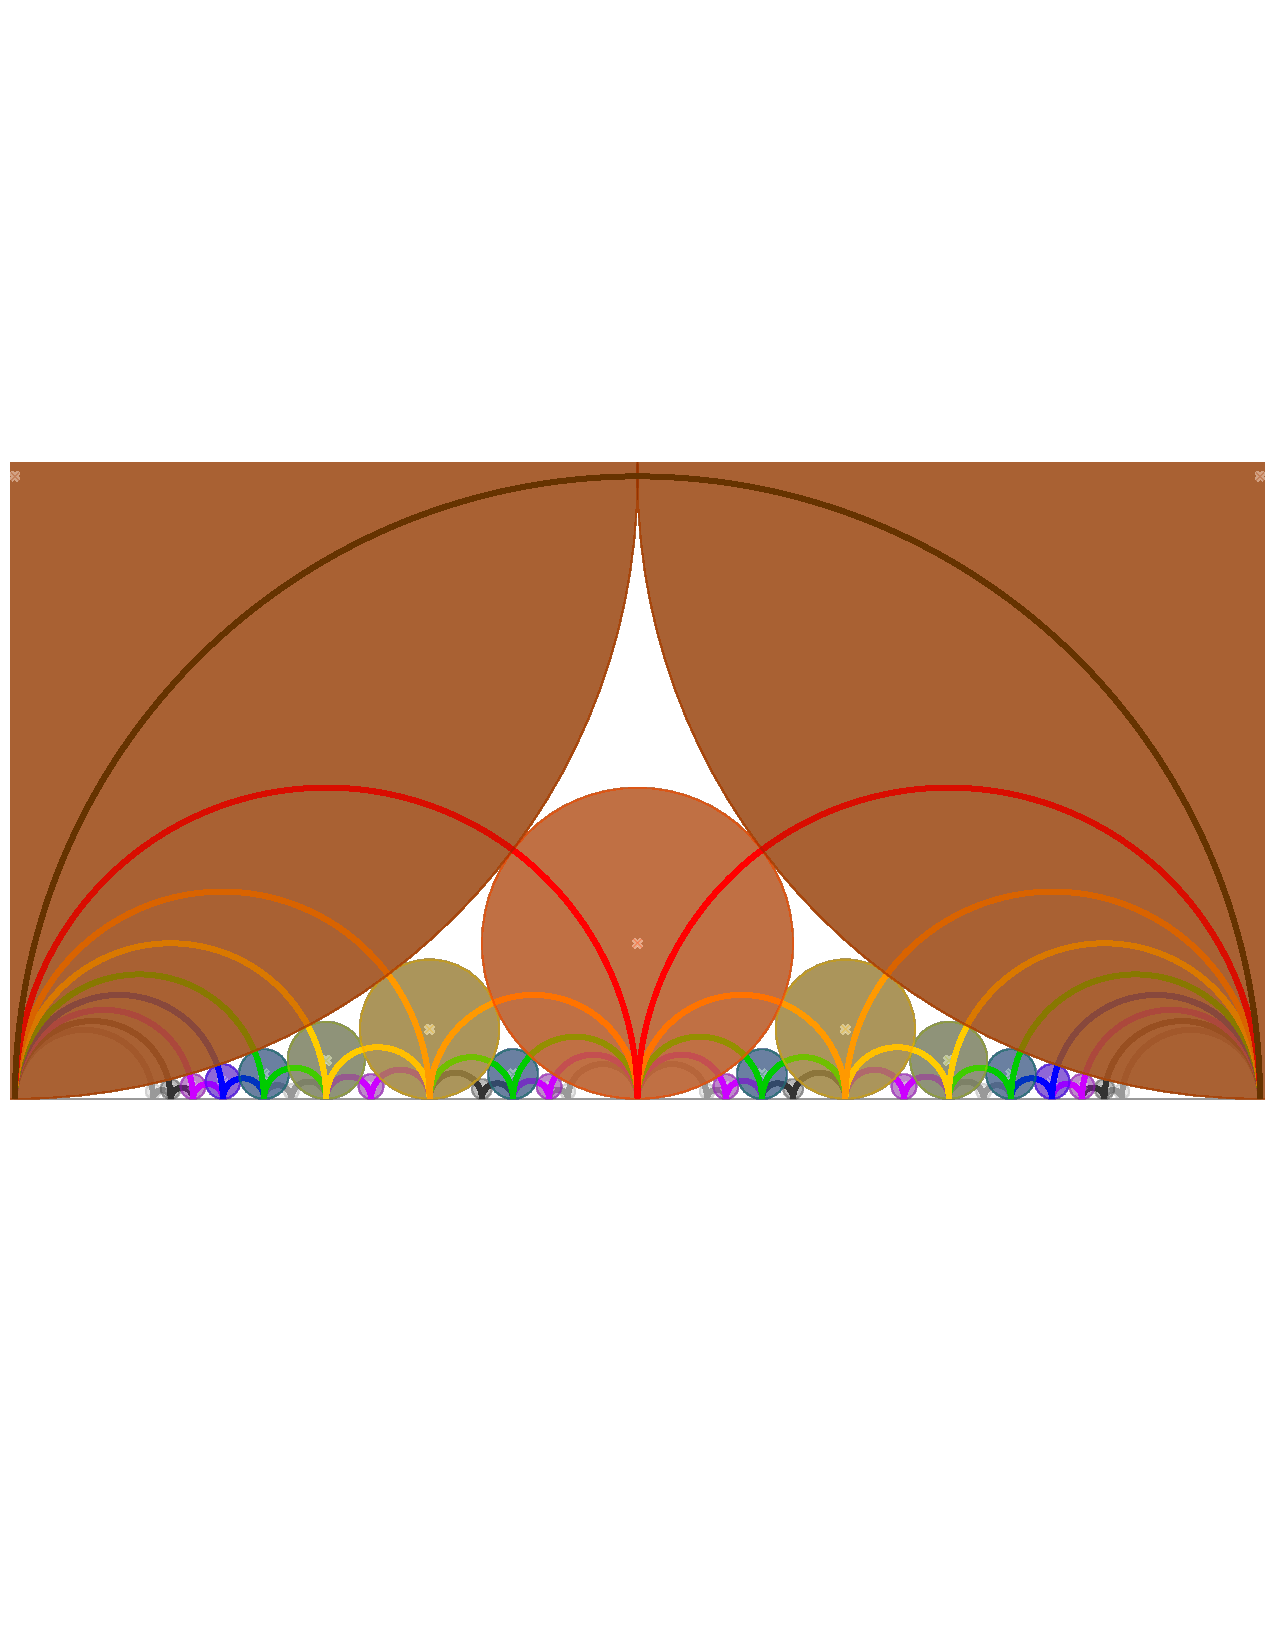
\includegraphics[width=\textwidth]{ford-circles.pdf}};
  % 分数 p/q 的切点位于图宽约 0.0033+0.9934*(p/q) 处
  \foreach \p/\q in {0/1, 1/6, 1/5, 1/4, 1/3, 2/5, 1/2, 3/5, 2/3, 3/4, 4/5, 5/6, 1/1}{
    \pgfmathsetmacro{\fx}{0.0033+0.9934*(\p/\q)}
    \coordinate (t) at ($(img.south west)!\fx!(img.south east)$);
    \draw[selvage, thin] (t) -- ++(0,-1.5pt);
    \node[below=3pt, font=\footnotesize] at (t) {$\frac{\p}{\q}$};
  }
\end{tikzpicture}
\caption{$F_1$ 至 $F_9$ 各分数的 Ford 圆与 Farey 弧线对照图。每个 Ford 圆与
$x$ 轴相切于对应分数处；两圆外切当且仅当对应分数是 Farey 邻项（定理
\ref{thm:ford}）。图中同色的半圆弧是 Farey 图中连接相邻分数的弧线，每条弧与
对应的 Ford 圆正交。原图底部的交互式标注在静态打印时会互相重叠，本笔记将其
隐去，改标 $F_6$ 的十三个分数（更密的标注在本图宽度下无法避免重叠，这正是
原图采用悬停交互的原因）。原图：CMG Lee，Wikimedia Commons，CC BY-SA 4.0
（有改动：去除标注层、转为 PDF 并裁剪）。}
\label{fig:ford}
\end{figure}

\begin{theorem}[Ford 圆与 Farey 邻项]\label{thm:ford}
两个不同的最简分数 $a/b<c/d$ 的 Ford 圆只可能相切或相离；它们相切，当且仅当
$|bc-ad|=1$，即两分数是 Farey 邻项。此时存在唯一的第三个 Ford 圆与两圆都相切，
它对应的分数恰是中位分数 $(a+c)/(b+d)$。
\end{theorem}

\begin{proof}
计算两圆心距离的平方与半径和、差的平方：
\[
  \Big(\frac ab-\frac cd\Big)^2+\Big(\frac{1}{2b^2}-\frac{1}{2d^2}\Big)^2
  =\Big(\frac{1}{2b^2}+\frac{1}{2d^2}\Big)^2+\frac{(bc-ad)^2-1}{b^2d^2}.
\]
两分数不同且都最简，故 $bc-ad$ 是非零整数，$|bc-ad|\ge1$，于是圆心距不小于半径
之和，即两圆相离或外切；取等号（外切）当且仅当 $|bc-ad|=1$，由定理
\ref{thm:farey-neighbor} 这等价于 Farey 邻项。相切时中位分数的圆与两者都相切
（因中位分数与每个端点都满足行列式 $1$ 的关系），唯一性由两圆公切圆在
$x$ 轴切点位置的唯一性给出。
\end{proof}

\subsection{递推关系}

Farey 序列可以自左向右递推生成，无需逐一插入。

\begin{proposition}[Farey 序列的三项递推]\label{prop:farey-recurrence}
设 $F_n$ 中相邻三项为 $\dfrac ab<\dfrac pq<\dfrac cd$，则存在整数 $k\ge1$ 使
\[
  a+c=kp,\qquad b+d=kq,
\]
且 $k$ 由
\[
  k=\Big\lfloor\frac{n+b}{q}\Big\rfloor
\]
唯一确定。由此，记 $F_n$ 的第 $i$ 项为 $p_i/q_i$，则
\[
  p_{i}=\Big\lfloor\frac{n+q_{i-2}}{q_{i-1}}\Big\rfloor p_{i-1}-p_{i-2},
  \qquad
  q_{i}=\Big\lfloor\frac{n+q_{i-2}}{q_{i-1}}\Big\rfloor q_{i-1}-q_{i-2},
\]
递推起点为 $(p_0,q_0)=(0,1)$，$(p_1,q_1)=(1,n)$。
\end{proposition}

\begin{proof}
由定理 \ref{thm:farey-neighbor}，相邻两对都满足行列式关系：
$bp-aq=1=cq-dp$，解出
\[
  \frac pq=\frac{a+c}{b+d}
\]
（中位分数关系，但 $a+c$ 与 $b+d$ 可能有公因子，故写成整数倍 $k$）。于是
$c=kp-a$，$d=kq-b$。$c/d$ 要落在 $F_n$ 中需 $d=kq-b\le n$，即
$k\le(n+b)/q$；而差值
\[
  \frac{kp-a}{kq-b}-\frac pq=\frac{bp-aq}{q(kq-b)}=\frac{1}{q(kq-b)}
\]
随 $k$ 增大而严格减小。$c/d$ 是 $p/q$ 在 $F_n$ 中的\emph{右邻}，即所有满足
$kq-b\le n$ 的候选中差值最小者，故应取最大的可行 $k$，即
$k=\lfloor(n+b)/q\rfloor$。代入 $c=kp-a$、$d=kq-b$ 得递推式；起点 $0/1$ 与
$1/n$ 是 $F_n$ 的前两项。
\end{proof}


\end{document}
